\documentclass[11pt]{scrartcl}

% Packages + configuration
% !TEX root = documentation.tex

%-------------------------
% imports
% ------------------------
\usepackage[utf8]{inputenc}
\usepackage[T1]{fontenc}
\usepackage[ngerman]{babel}
\usepackage[left=3cm,top=2.5cm,right=2.5cm,bottom=2cm]{geometry}
\usepackage{microtype}
\usepackage{amsmath}
\usepackage{graphicx}
\usepackage{booktabs}
\usepackage{array}
\usepackage{enumitem}
\usepackage{hyperref}
\usepackage{tikz}
\usepackage{abstract}
\usepackage[natbibapa]{apacite}
\usepackage{tabularx}
\usepackage[affil-it]{authblk}
\usepackage{newtxtext}
\usepackage{newtxmath}
\usepackage{multicol}
\setkomafont{disposition}{\bfseries}
\usepackage{float}
\usetikzlibrary{arrows.meta,positioning,shapes.geometric}


%-------------------------
% configuration
% ------------------------

% paragraph indent
\setlength{\parindent}{0pt}

% hyperlink colors
\hypersetup{
         colorlinks,
         citecolor=black,
         filecolor=black,
         linkcolor=black,
         urlcolor=black,
         pdfborder=0 0 0
}

\bibliographystyle{apacite}


\begin{document}
% !TEX root = documentation.tex


\titlehead{BSc Computational and Data Science\\CDS-309 Hyperautomation und RPA\\Dozenten: Markus Müntener, Matthias Müller\hfill}
\title{Automatisierung eines Moodle-basierten Lernplanungsprozesses mit UiPath und generativer KI}
\author[1,*]{Alessio De Icco}
\author[2,*]{Florin Gartmann}
\author[3,*]{Michal Karczmarzyk}
\author[4,*]{Oliver Schütz}
\affil[1]{Fachhochschule Graubünden}
\affil[*]{E-Mail Adressen: michal.karczmarzyk@stud.fhgr.ch, oliver.schuetz@stud.fhgr.ch, alessio.deicco@stud.fhgr.ch, florin.gartmann@stud.fhgr.ch}
\date{\today}
\maketitle

\begin{abstract}
Diese Arbeit untersucht die Automatisierung eines Moodle-basierten Lernplanungsprozesses mit UiPath, Moodle-Datenzugriff und generativer KI. Ausgangspunkt ist das Problem, dass Studierende Kursinformationen, Aufgaben, Deadlines und Semesterunterlagen häufig manuell in verschiedenen Moodle-Kursen suchen und anschliessend für die Erstellung eines Lernplans aufbereiten müssen.

Ziel des Moodle-to-LLM Study Planners ist es, diese wiederkehrenden Arbeitsschritte zu automatisieren. UiPath steuert den Prozess, liest relevante Moodle-Informationen aus, speichert sie strukturiert zwischen und übergibt sie an die Gemini API, die daraus einen Lernplan erstellt. Damit verbindet die Lösung klassische RPA mit API-Nutzung und GenAI zu einem Hyperautomation-Ansatz.

Die Analyse zeigt, dass der Prozess technisch gut automatisierbar ist, da er digital, wiederholbar und datengetrieben abläuft. Herausforderungen bestehen vor allem in uneinheitlichen Moodle-Strukturen, unterschiedlichen PDF-Formaten, API-Fehlern und der Validierung von LLM-Antworten. Durch strukturierte Datenverarbeitung, Logging und Retry-Mechanismen können diese Risiken reduziert werden. Insgesamt zeigt die Arbeit, dass der gewählte Prozess sowohl fachlich relevant als auch technisch und ökonomisch für eine RPA-Automatisierung geeignet ist.
\end{abstract}

\clearpage

\newpage
\tableofcontents
\newpage

\section{Einleitung und Prozessbeschreibung}
\subsection{Ausgangslage}
Im Studienalltag sind relevante Informationen nicht an einem einzigen, standardisierten Ort gebündelt. Aufgaben, Deadlines, Semesterinformationen, Folien, Übungsblätter und organisatorische Hinweise verteilen sich über verschiedene Moodle-Kurse, die jede Dozentin und jeder Dozent anders strukturiert. Wer daraus einen Lernplan ableiten möchte, muss jeden Kurs einzeln öffnen, die passenden Dokumente suchen, Termine heraussuchen, Inhalte kopieren und sie schliesslich von Hand in ein Werkzeug wie ChatGPT oder Gemini übertragen.

Für eine RPA-Gruppenarbeit eignet sich dieser Prozess besonders, weil er fachlich relevant ist und zugleich typische Automatisierungsfragen aufwirft: Der Ablauf ist wiederkehrend, regelbasiert und digital, enthält mit PDF-Dokumenten und natürlichsprachlichen Kursinformationen aber auch unstrukturierte Anteile. Damit ist er weder trivial noch übermässig komplex und lässt sich nutzen, um Prozessanalyse, technische Qualifikation, Wirtschaftlichkeit, UiPath-Umsetzung und den Einsatz generativer KI an einem durchgehenden Beispiel zu untersuchen.

\subsection{Zielsetzung und Forschungsfrage}
Ziel der Lösung ist ein automatisierter Lernplanungsprozess, der aktuelle Moodle-Informationen sammelt, strukturiert, an ein LLM übergibt und das Ergebnis als fertigen Lernplan ausgibt. Daraus leitet sich die folgende Leitfrage ab: \emph{Wie kann ein Moodle-basierter Lernplanungsprozess durch RPA, API-Nutzung und generative KI so automatisiert werden, dass wiederkehrende manuelle Arbeit reduziert und Studieninformationen zuverlässiger nutzbar werden?}

Der Nutzen liegt auf drei Ebenen: Die Lösung senkt den manuellen Aufwand, indem sie wiederkehrende Such-, Kopier- und Strukturierungsarbeiten automatisiert; sie schafft mehr Übersicht über Kurse, Deadlines und Lernaufwand; und sie liefert ein einheitliches Ausgabeformat, obwohl die Eingaben aus verschiedenen Kursen und Dateitypen stammen.

\subsection{Was ist RPA und wie funktioniert es im Prinzip?}
Robotic Process Automation bezeichnet die Automatisierung digitaler, regelbasierter Tätigkeiten durch Software-Roboter. Ein Bot kann etwa Applikationen öffnen, Felder ausfüllen, Dateien lesen, Daten transformieren, APIs ansprechen sowie Ergebnisse speichern oder versenden. Anders als die klassische Softwareentwicklung setzt RPA dabei auf bestehende Arbeitsabläufe und nutzt deren vorhandene Benutzeroberflächen und Schnittstellen.

Im vorliegenden Projekt geht RPA über diesen Rahmen hinaus: Der Bot führt nicht bloss Klick- und Kopieraktionen aus, sondern verknüpft Moodle-Daten, API-Aufrufe, lokale Datenstrukturen, Validierung und LLM-Verarbeitung. Diese Kombination ist charakteristisch für Hyperautomation und steigert den Nutzen, weil nicht nur ein einzelner Handgriff ersetzt, sondern ein ganzer Informationsprozess vom Auslesen bis zum fertigen Lernplan automatisiert wird.

\subsection{Beschreibung des Prozesses}
Der Ist-Prozess entspricht dem eingangs geschilderten manuellen Vorgehen in Moodle. Der Soll-Prozess startet dagegen per Benutzer-Trigger in UiPath: Der Bot lädt Konfiguration und Zugangsdaten, liest die Moodle-Kurse aus und filtert sie nach Semester, verarbeitet Kursinformationen und Semester-PDFs, bereinigt die Rohdaten, übergibt sie an Gemini, validiert das Ergebnis und speichert es als Lernplan. Abschliessend werden die erzeugten Lernpläne zu PDF-Berichten gebündelt und der Nutzerin oder dem Nutzer per E-Mail zugestellt. Die einzelnen Schritte werden in Abschnitt~\ref{sec:automatisierungsschritte} im Detail beschrieben.

\subsection{Manuelle Durchführung als Referenzprozess}
Die folgenden Screenshots veranschaulichen den oben beschriebenen manuellen Referenzprozess in Moodle: vom Öffnen des Kurses über das Sichten der Materialien und Fristen bis zum daraus erstellten Lernplan, den die Automatisierung fachlich ersetzt.

\begin{figure}[H]
\centering
\begin{minipage}[t]{0.48\textwidth}
\centering

\includegraphics[width=\textwidth]{images/manual-process/01-moodle-kursstart.png}
\end{minipage}\hfill
\begin{minipage}[t]{0.48\textwidth}
\centering
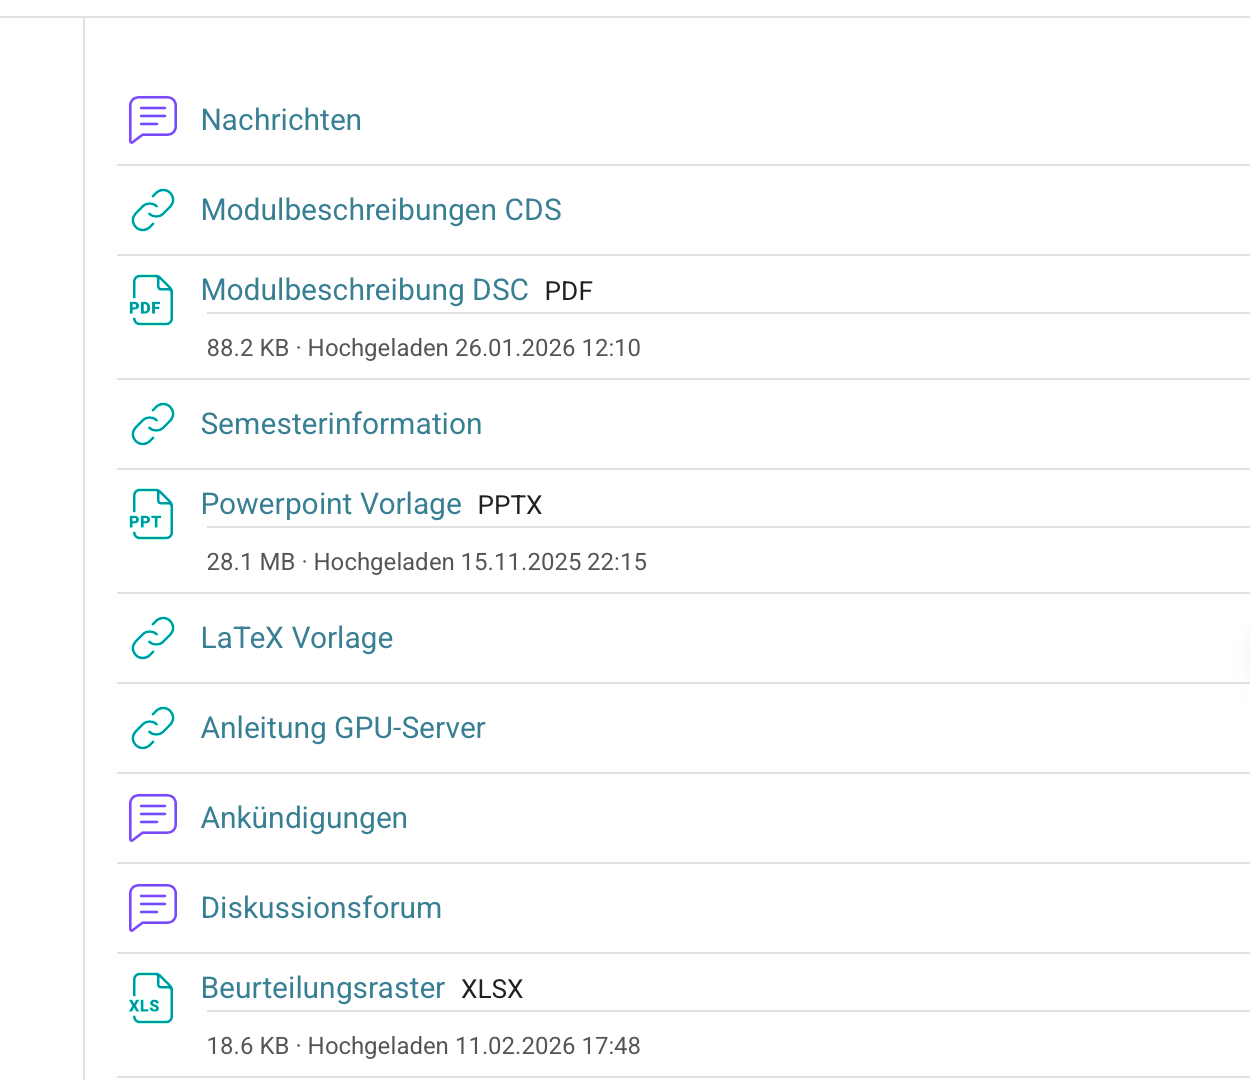
\includegraphics[width=\textwidth]{images/manual-process/02-kursmaterialien.png}
\end{minipage}

\vspace{0.45cm}

\begin{minipage}[t]{0.48\textwidth}
\centering
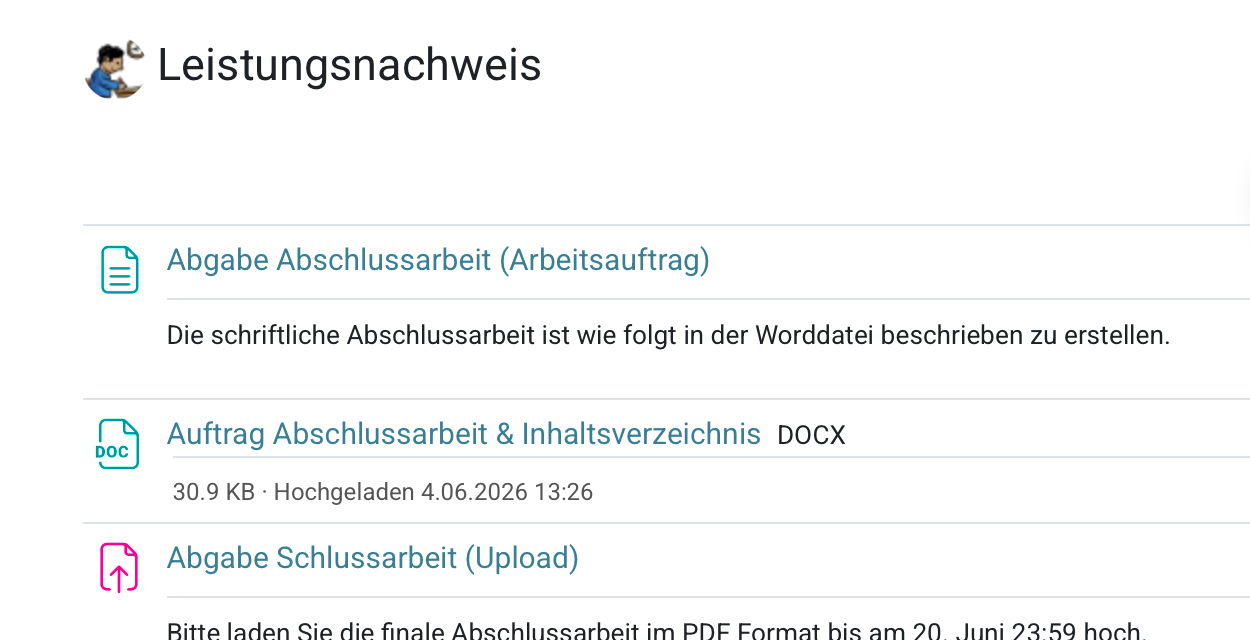
\includegraphics[width=\textwidth]{images/manual-process/03-abgabe-und-deadline.png}
\end{minipage}\hfill
\begin{minipage}[t]{0.48\textwidth}
\centering
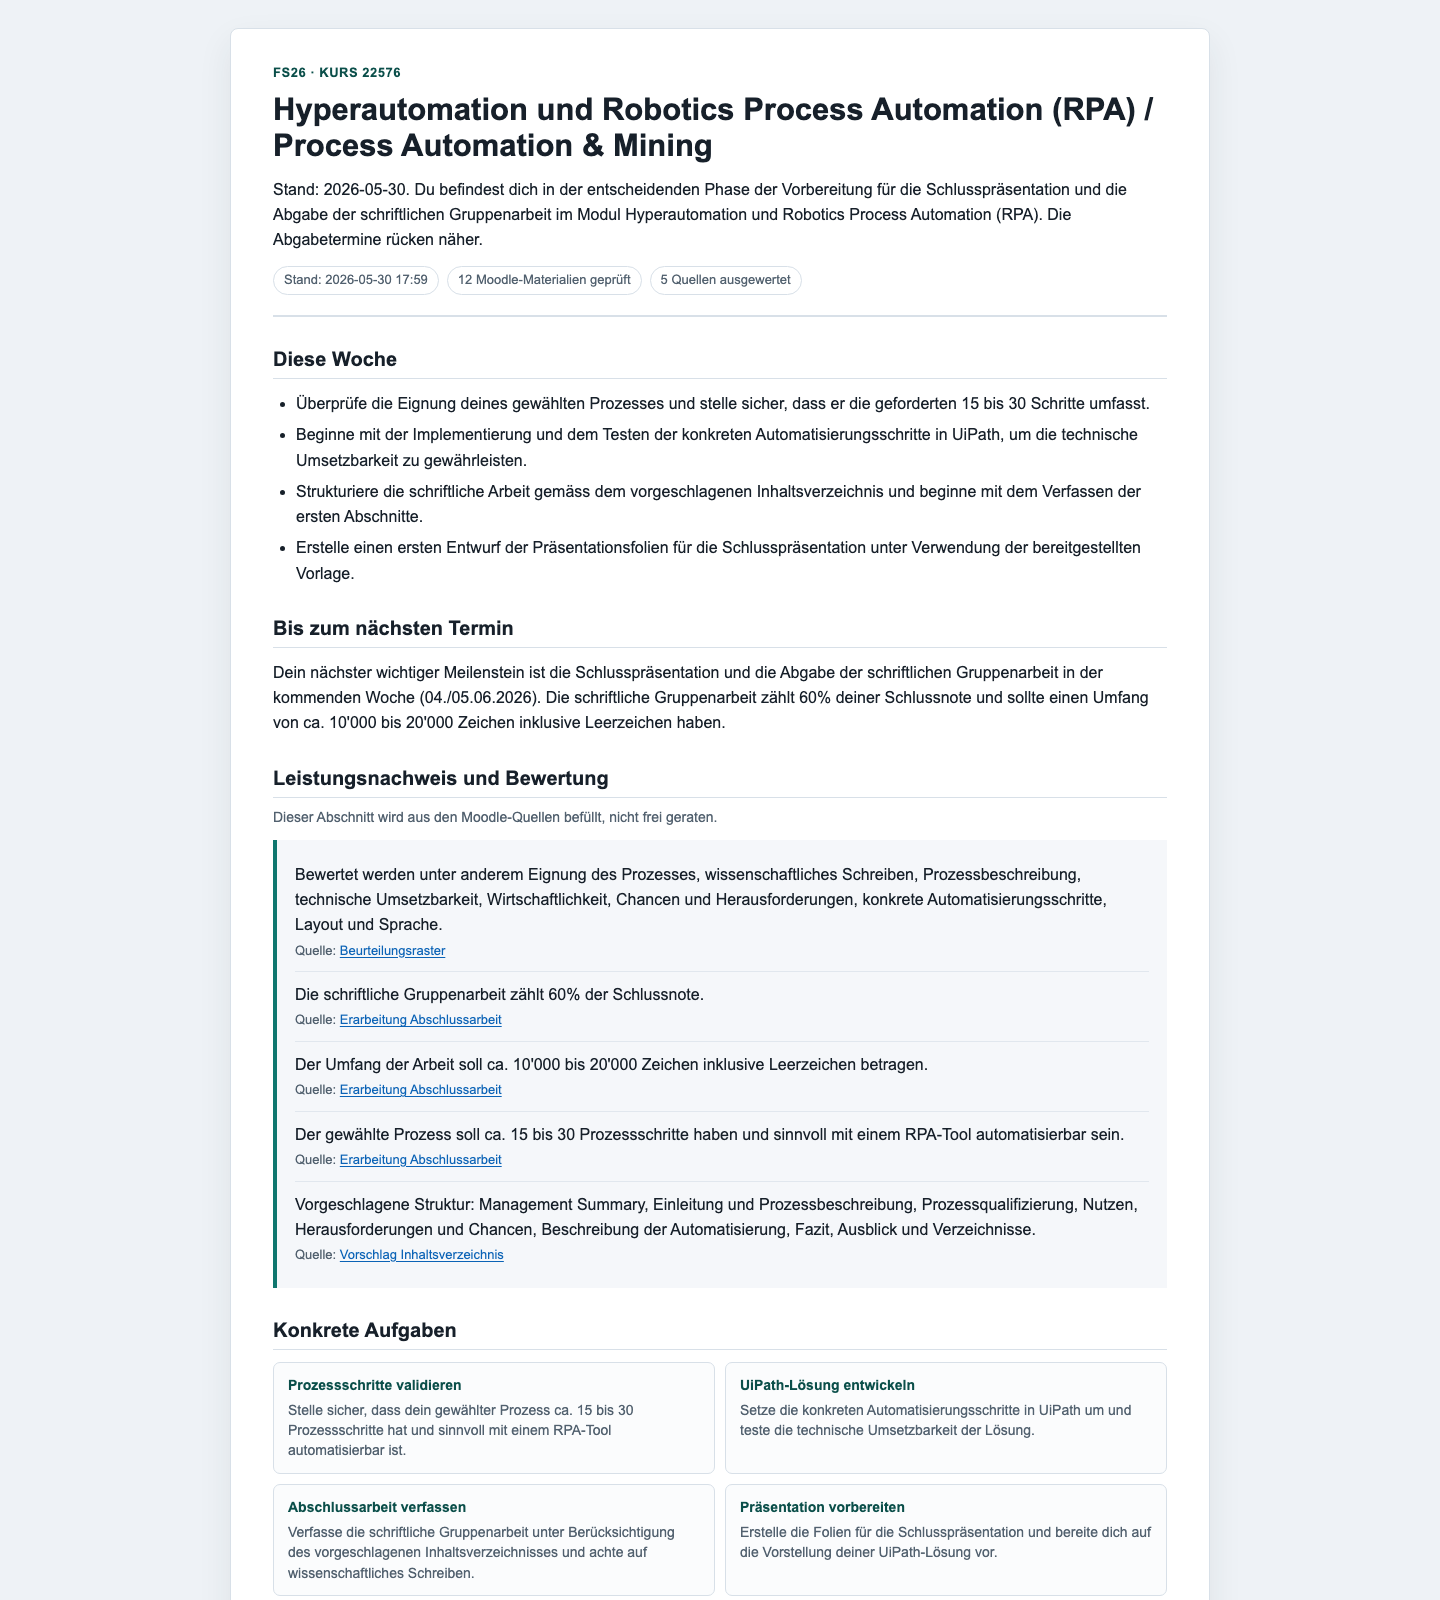
\includegraphics[width=0.78\textwidth]{images/manual-process/04-generierter-lernplan.png}
\end{minipage}
\caption{Screenshots des manuellen Referenzprozesses und des Zielergebnisses}
\end{figure}

\section{Prozessqualifizierung}
Die Evaluation des vorgeschlagenen Prozesses \textit{Moodle-to-LLM Study Planner} folgt einer zweistufigen Qualifizierungsmethodik, die auf den standardisierten Kriterien des Process Qualification Document (PQD) beruht. Geprüft wird der Prozess dabei nacheinander auf seine technische Machbarkeit und auf seine ökonomische Sinnhaftigkeit (Business Case und Return on Investment).
\subsection{Technische Eignung}
Technisch ist der Prozess für eine Automatisierung gut geeignet, weil alle Kernaktivitäten digital ablaufen. Moodle bildet die primäre Datenquelle, die Verarbeitung erfolgt lokal in strukturierten Formaten wie JSON oder Text, und Gemini ist über eine API angebunden. UiPath Studio steuert den Ablauf und deckt Logging, Fehlerbehandlung, Dateizugriffe, HTTP-Requests und Prozessschleifen ab. Besonders vorteilhaft ist, dass der Prozess für die Datenbeschaffung nicht auf fragile UI-Klicks angewiesen ist: Wo möglich, liest der Bot die Moodle-Daten über API- oder CLI-Zugriff aus, was die Lösung stabiler macht als reines Screen-Scraping. Eine Ausnahme bildet der Login: Hier füllt der Bot das Anmeldeformular im Browser klassisch über Klick- und Eingabeaktionen aus; erst die anschliessende Datenverarbeitung läuft über API beziehungsweise CLI.

Zugleich besitzt der Prozess genügend Komplexität, um RPA-Kompetenzen nachzuweisen: Er umfasst Konfiguration, Credentials, Session-Handling, Kursfilterung, Schleifen über mehrere Kurse, unstrukturierte PDF-Inhalte, LLM-Kommunikation, Validierung, Retry-Logik, Report-Erstellung und Abschlusskommunikation. Damit geht er deutlich über eine einfache Makro-Automatisierung hinaus.

\subsection{Ökonomische Qualifizierung und Business Case}
Die ökonomische Evaluation orientiert sich an den theoretischen Vorgaben zur Aufwands- und Nutzenbestimmung von \cite{Wanner2019} sowie \cite{Beetz2019}. Zur Ermittlung der Wirtschaftlichkeit (Return on Investment, ROI) wird der eingesparte manuelle Aufwand den Implementierungs- und Betriebskosten gegenübergestellt. Dabei sind zwei Einsatzszenarien zu unterscheiden, die sich im Kostenbild deutlich unterscheiden: Im ersten betreibt eine einzelne studierende Person die Lösung mit kostenlosen Werkzeugen für sich selbst; im zweiten stellt die Hochschule den Prozess als zentralen Dienst für einen ganzen Jahrgang bereit, wodurch kostenpflichtige Lizenzen, API-Nutzung und Wartung hinzukommen. Da der Nutzen in beiden Szenarien identisch ist, wird er vorab bestimmt.

\subsubsection{Analyse des Einsparpotenzials (Nutzen-Dimension)}
Gemäss dem vorliegenden Solution Design Document (SDD) -- der technischen Spezifikation, in der wir Prozessablauf, Architektur und Aktivitäten der Lösung festgehalten haben -- dauert das manuelle Suchen, Extrahieren und Aufbereiten der Kursdaten im Durchschnitt 15 Minuten pro Fall. Geht man konservativ von rund 3 solchen Fällen pro Woche und einer regulären Semesterdauer von 14 Wochen aus, ergibt sich pro Studierende:r das folgende quantitative Einsparpotenzial:

\begin{equation}
\begin{split}
\text{Automatisierbarer Aufwand} &= 3 \text{ Fälle/Woche} \cdot 15 \text{ Min./Fall} \cdot 14 \text{ Wochen} \\
&= 630 \text{ Minuten} \ (\mathbf{10{,}5 \text{ Stunden/Semester}})
\end{split}
\end{equation}

Studierende werden für ihren Studienaufwand zwar nicht entlöhnt, doch ihre Zeit besitzt dennoch einen ökonomischen Wert. Dieser wird über Opportunitätskosten abgebildet, also über den Nutzen, der entgeht, weil die Zeit nicht anderweitig -- etwa für einen studentischen Nebenjob oder vertieftes Lernen -- eingesetzt werden kann. Der angesetzte Satz von CHF 20.-- pro Stunde orientiert sich an einem typischen studentischen Nebenverdienst und macht die eingesparte Zeit monetär vergleichbar. Daraus resultiert ein individueller monetärer Nutzen von \textbf{rund CHF 210.-- pro Semester} und Studierendem. Über einen gesamten Studiengangsjahrgang von rund 30 Studierenden summiert sich die eingesparte Zeit auf etwa 315 Stunden bzw. einen Gesamtnutzen von \textbf{rund CHF 6'300.-- pro Semester}.

\subsubsection{Szenario 1: Nutzung durch einzelne Studierende}
In diesem Szenario betreibt eine studierende Person die Automatisierung eigenständig auf dem eigenen Rechner. Zum Einsatz kommen die kostenlose UiPath Community Edition, das Free-Tier der Gemini-API und die lokale Ausführung; die laufenden Kosten betragen damit praktisch null (Tabelle~\ref{tab:betriebskosten}).

\begin{table}[ht]
\centering
\caption{Laufende monatliche Betriebskosten im studentischen Self-Service}
\label{tab:betriebskosten}
\begin{tabularx}{\textwidth}{@{}Xr@{}}
\toprule
\textbf{Kostenkomponente} & \textbf{Kosten pro Monat} \\
\midrule
UiPath Community Edition (Einzelnutzung) & CHF 0.-- \\
Gemini API (Free Tier) & CHF 0.-- \\
Lokale Ausführung (eigener Rechner) & CHF 0.-- \\
\midrule
\textbf{Gesamtkosten pro Monat} & \textbf{$\approx$ CHF 0.--} \\
\bottomrule
\end{tabularx}
\end{table}

Da keine laufenden Kosten anfallen, beschränkt sich der Aufwand auf die einmalige Entwicklung der Lösung, die im Rahmen dieses Projekts bereits erbracht wurde. Für die einzelne Person ist dieser Aufwand somit vernachlässigbar, während ihr ein wiederkehrender Nutzen von rund CHF 210.-- pro Semester gegenübersteht. Im Self-Service ist die Lösung damit faktisch sofort wirtschaftlich.

\subsubsection{Szenario 2: Bereitstellung durch die Hochschule}
Stellt die Hochschule den Prozess als zentralen Dienst für einen ganzen Jahrgang bereit, ändert sich das Kostenbild grundlegend. Die UiPath Community Edition ist für den organisationsweiten, produktiven Einsatz nicht lizenziert, und das kostenlose Gemini-Kontingent genügt für das Volumen mehrerer Dutzend Studierender nicht mehr. Es fallen daher kostenpflichtige UiPath-Lizenzen sowie eine bezahlte Nutzung der Gemini-API an. Hinzu kommt der laufende Betrieb: Eine zentral bereitgestellte Lösung muss von einer mitarbeitenden Person gewartet werden, etwa für Updates, Fehlerbehebung und die Anpassung an Änderungen in Moodle.

Bevor diese laufenden Kosten entstehen, muss das Tool jedoch zunächst einmalig entwickelt werden. Tabelle~\ref{tab:entwicklungskosten} stellt dem RPA-Ansatz in UiPath bewusst eine klassische, native Code-Lösung gegenüber. Diese Gegenüberstellung dient nicht als blosses Negativbeispiel: Eine native Entwicklung bietet durchaus eigene Vorteile -- etwa die volle Kontrolle über den Quellcode, eine potenziell höhere Performance, geringere Abhängigkeit von Lizenzanbietern sowie flexiblere Integrationsmöglichkeiten -- und sollte daher als ernsthafte Option in die Technologieentscheidung einbezogen werden.

\begin{table}[ht]
\centering
\caption{Einführungs-/Entwicklungskosten: native Code-Lösung vs. UiPath}
\label{tab:entwicklungskosten}
\begin{tabularx}{\textwidth}{@{}l *{2}{>{\centering\arraybackslash}X}@{}}
\toprule
\textbf{Kriterium} & \textbf{Klassische Code-Lösung} & \textbf{UiPath-Automatisierung} \\
\midrule
Geschätzter Entwicklungsaufwand & 30 Stunden & 12 Stunden \\
Interner Lohnwert (CHF 40.--/h) & CHF 1'200.-- & CHF 480.-- \\
Marktüblicher Verkaufspreis (CHF 150.--/h) & CHF 4'500.-- & CHF 1'800.-- \\
\bottomrule
\end{tabularx}
\end{table}

Der Einsatz von UiPath senkt den einmaligen Entwicklungsaufwand somit deutlich um 18 Stunden bzw. 60\,\% (von CHF 1'200.-- auf CHF 480.-- internem Lohnwert). Als Alternative käme eine Low-Code-Plattform wie Microsoft Power Automate in Frage, die über bestehende Microsoft-365-Bildungslizenzen häufig bereits abgedeckt ist; die Wahl von UiPath erfolgte hier primär aus didaktischen Gründen.

Unabhängig von der gewählten Technologie stellt sich zudem die grundsätzliche Make-or-Buy-Frage. Verfügt die Hochschule über die nötigen Entwicklungskompetenzen und freie personelle Ressourcen, lässt sich die Lösung in-house realisieren -- mit den oben ausgewiesenen Kosten und voller Kontrolle über Wartung und Weiterentwicklung. Fehlen diese Kompetenzen oder Kapazitäten, kann die Automatisierung stattdessen extern als Individualsoftware eingekauft werden. Dies verlagert den Entwicklungsaufwand auf einen Dienstleister, schlägt sich aber im marktüblichen Verkaufspreis (Tabelle~\ref{tab:entwicklungskosten}) nieder und schafft eine gewisse Abhängigkeit bei künftigen Anpassungen und beim Support.

Zusammen mit den laufenden Lizenz-, API- und Wartungskosten ergibt sich für den Hochschulbetrieb das in Tabelle~\ref{tab:betriebskosten-hochschule} dargestellte Kostenbild.

\begin{table}[ht]
\centering
\caption{Kostenbild im Hochschulbetrieb (Schätzwerte)}
\label{tab:betriebskosten-hochschule}
\begin{tabularx}{\textwidth}{@{}Xr@{}}
\toprule
\textbf{Kostenkomponente} & \textbf{Kosten} \\
\midrule
Entwicklung (einmalig, via UiPath) & CHF 480.-- einmalig \\
UiPath-Lizenzierung (Basic-Tier, ca. CHF 25.--/Monat) & ca. CHF 300.--/Jahr \\
Gemini API (kostenpflichtig, Jahrgang) & ca. CHF 200.--/Jahr \\
Wartung ($\approx$ 2 h/Monat à CHF 40.--) & ca. CHF 1'000.--/Jahr \\
\midrule
\textbf{Laufende Kosten gesamt} & \textbf{ca. CHF 1'500.--/Jahr} \\
\bottomrule
\end{tabularx}
\end{table}

Wichtig ist dabei, dass für diesen geringen, periodisch laufenden Workload keine teure Enterprise-Lizenzierung mit dediziertem \textit{Unattended Robot} (bis zu CHF 13'000.--/Jahr) nötig ist: Ein zentraler, schlanker Betrieb lässt sich bereits mit dem UiPath Basic-Tier ab ca. CHF 25.-- pro Monat abdecken. Den laufenden Kosten von rund CHF 1'500.-- pro Jahr (zuzüglich der einmaligen Entwicklung von CHF 480.--) steht ein jährlicher Bruttonutzen von rund CHF 12'600.-- pro Jahrgang gegenüber (CHF 6'300.-- pro Semester). Die Lösung ist somit auch im Hochschulbetrieb bereits im ersten Jahr klar wirtschaftlich. Da die Fixkosten -- Entwicklung, Wartung und Lizenz -- weitgehend unabhängig von der Nutzerzahl sind, verbessert sich die Wirtschaftlichkeit mit jeder weiteren nutzenden Person zusätzlich (Skaleneffekt).

Insgesamt qualifiziert sich der Prozess damit in beiden Szenarien als wirtschaftlich attraktive Automatisierung: im Self-Service praktisch kostenlos und sofort rentabel, im Hochschulbetrieb dank schlanker Lizenzierung bereits im ersten Jahr -- eine \textit{Low Hanging Fruit} mit geringer Komplexität und hohem Wertbeitrag (\textit{Best Value}).

\section{Beschreibung der Automatisierung}
\subsection{Kernanwendungen und Architektur}
Die Lösung ruht auf vier Kernbausteinen: UiPath Studio dient als Entwicklungsumgebung und Execution Engine, Moodle als Datenquelle für Kurse, Aufgaben und Semesterinformationen. Die extrahierten Rohdaten werden lokal in JSON- oder Textdateien zwischengespeichert, bevor Gemini sie zu einem Lernplan verarbeitet.

Der Ablauf folgt einem API-first-Ansatz, ergänzt durch eine RPA-Orchestrierung. In einer frühen Projektphase hatten wir geplant, den gesamten Zugriff -- inklusive Datenabruf -- über klassische Browseraktionen abzuwickeln. Im finalen SDD beschränken sich solche Browseraktionen wie \texttt{Open Browser}, \texttt{Type Into Username}, \texttt{Type Into Password} und \texttt{Click Login} dagegen auf den Login, der sich nicht über eine API abbilden lässt; das eigentliche Auslesen der Daten haben wir auf Moodle CLI/API und einen Docker-Container umgestellt. Diese Entwicklung ist sinnvoll: Für Login und Bedienung ist UI-Automatisierung zwar anschaulich, doch beim wiederholten Auslesen von Daten sind APIs stabiler, schneller und besser testbar. UiPath bleibt dennoch zentral, weil es Trigger, Konfiguration, Ablaufsteuerung, Logging, Dateiverarbeitung, HTTP-Requests und Fehlerbehandlung zusammenführt.

\subsection{Automatisierungsschritte}
\label{sec:automatisierungsschritte}
Abbildung~\ref{fig:bpmn} fasst den gesamten Ablauf im Überblick zusammen; im Folgenden werden die einzelnen Schritte erläutert. Der Prozess startet manuell per Tastendruck in UiPath. Ein zeitgesteuerter Trigger wurde bewusst verworfen, weil Lernpläne meist genau dann gebraucht werden, wenn Studierende aktiv nach Kursaktualisierungen suchen. Nach dem Start lädt der Bot Konfigurationswerte wie Moodle-URL, Output-Pfad, Semesterkennung und API-Endpunkte. Zugangsdaten sind nicht im Workflow hart codiert, sondern liegen in Umgebungsvariablen oder einem Credential Store, etwa \texttt{MOODLE\_USERNAME}, \texttt{MOODLE\_PASSWORD} und ein Gemini-API-Key.

Anschliessend prüft der Bot die Moodle-Session und meldet sich bei ungültiger Sitzung neu an. Danach liest er die Kursliste aus Moodle und verarbeitet sie als JSON. Die Kurse filtert er nach der aktuellen Semesterkategorie, beispielsweise FS26, und prüft für jeden, ob relevante Details vorhanden sind, darunter Kursname, Kurslink, Aufgaben, Beschreibungen, Abgabedaten und Links auf Semesterinformationen. Findet er ein Semesterinformations-PDF, extrahiert er dessen Inhalt und ergänzt damit die Rohdaten.

Nach dem Scraping folgt die Datenbereinigung: HTML-Tags, überflüssige Leerzeichen und uneinheitliche Datumsformate werden entfernt oder vereinheitlicht. Daraus baut UiPath eine strukturierte Datentabelle beziehungsweise ein JSON-Objekt auf. Die anschliessende Validierung prüft, ob Aufgaben vorhanden sind, ob Deadlines fehlen und ob zentrale Felder leer geblieben sind. Erst dann entsteht der Prompt. Er muss kompakt genug für das Token-Limit bleiben, zugleich aber genügend Kontext bieten, damit das LLM einen brauchbaren Lernplan erstellen kann.

Der API-Aufruf an Gemini liefert eine Antwort, die ihrerseits validiert wird. Ein einfaches Kriterium ist die Mindestlänge des Ergebnisses; zusätzlich lassen sich Pflichtbestandteile wie Kursname, Deadline, empfohlene Lernaktivität und Priorität prüfen. Ist die Antwort ungültig, wiederholt der Bot den Request bis zu drei Mal; bleibt sie auch dann ungültig, loggt er einen Fehler und markiert den betroffenen Kurs als Ausnahme. Bei gültigem Ergebnis erstellt er einen PDF-Report. Nach jedem Kurs kehrt der Prozess zur Frage zurück, ob ein weiterer Kurs vorliegt. Sind alle Kurse verarbeitet, schreibt der Bot eine Abschluss-E-Mail und beendet den Prozess.

\begin{figure}[H]
\centering
\resizebox{0.96\textwidth}{!}{%
\begin{tikzpicture}[
  task/.style={rectangle,rounded corners,draw,align=center,minimum width=2.85cm,minimum height=0.76cm,font=\scriptsize},
  event/.style={ellipse,draw,align=center,minimum width=1.5cm,minimum height=0.66cm,font=\scriptsize},
  gate/.style={diamond,draw,aspect=2.0,align=center,inner sep=1pt,font=\scriptsize},
  arrow/.style={-{Latex[length=1.6mm,width=1.3mm]},thick,shorten >=1pt,shorten <=1pt},
  looparrow/.style={-{Latex[length=1.6mm,width=1.3mm]},thick,rounded corners=4pt,shorten >=1pt,shorten <=1pt}
]

% Hauptpfad: Initialisierung, Kursverarbeitung und Speichern
\node[event] (start) at (0,0) {Start};
\node[task] (scope) at (0,-1.35) {Empfänger, Semester\\und Filter laden};
\node[task] (access) at (0,-2.70) {Moodle-Zugriff\\prüfen};
\node[task] (courses) at (0,-4.05) {Kurse für Semester\\abrufen};
\node[gate] (next) at (0,-5.65) {weiterer\\Kurs?};
\node[task] (course) at (0,-7.25) {Nächsten Moodle-\\Kurs auswählen};
\node[task] (resources) at (0,-8.60) {Ressourcenliste des\\Kurses abrufen};
\node[task] (semester) at (0,-9.95) {Semesterinfo aus\\Ressourcen finden};
\node[task] (deadlines) at (0,-11.30) {Abgaben, Termine\\und Prüfungen lesen};
\node[task] (topics) at (0,-12.65) {Themenblöcke und\\Aufwand erfassen};
\node[task] (priority) at (0,-14.00) {Lernschwerpunkte\\und Reihenfolge ableiten};
\node[task] (prompt) at (0,-15.10) {Prompt an Gemini\\senden};
\node[gate] (valid) at (0,-17.00) {Antwort\\lang genug?};
\node[task] (take) at (0,-18.65) {Lernplan aus\\Antwort übernehmen};
\node[task] (save) at (0,-20.00) {Lernplan als\\Markdown speichern};
\node[task] (done) at (0,-21.35) {Kurs abschließen};

% Retry-Ast: nur gleicher Aufruf, keine Prompt-Anpassung
\node[gate] (retry) at (5.4,-17.00) {Retry\\$< 3$?};
\node[task] (repeat) at (5.4,-15.10) {Gemini-Aufruf\\wiederholen};
\node[task] (error) at (5.4,-21.35) {Kurs als fehlerhaft\\loggen};

% Abschluss nach dem letzten Kurs
\node[task] (collect) at (4.9,-5.65) {Alle Markdown-\\Lernpläne sammeln};
\node[task] (render) at (8.7,-5.65) {HTML/PDF-Berichte\\erzeugen};
\node[task] (mail) at (12.5,-5.65) {PDFs als E-Mail-\\Anhang versenden};
\node[event] (end) at (15.8,-5.65) {Ende};

% Initialisierung und Kursdaten
\draw[arrow] (start) -- (scope);
\draw[arrow] (scope) -- (access);
\draw[arrow] (access) -- (courses);
\draw[arrow] (courses) -- (next);
\draw[arrow] (next) -- node[right,font=\scriptsize]{ja} (course);
\draw[arrow] (resources) -- (semester);
\draw[arrow] (semester) -- (deadlines);
\draw[arrow] (deadlines) -- (topics);
\draw[arrow] (topics) -- (priority);
\draw[arrow] (course) -- (resources);
\draw[arrow] (priority) -- (prompt);

% KI und Validierung
\draw[arrow] (prompt) -- (valid);
\draw[arrow] (valid) -- node[right,font=\scriptsize]{ja} (take);
\draw[arrow] (take) -- (save);
\draw[arrow] (valid.east) -- node[above,font=\scriptsize]{nein} (retry.west);
\draw[arrow] (retry) -- node[right,font=\scriptsize]{ja} (repeat);
\draw[arrow] (repeat.west) -- (prompt.east);
\draw[arrow] (retry) -- node[right,font=\scriptsize]{nein} (error);
\draw[arrow] (save) -- (done);
\draw[arrow] (error.west) -- (done.east);

% Kursabschluss und Abschlussprozess
\draw[looparrow] (done.west) -- ++(-2.15,0) |- (next.west);
\draw[arrow] (next.east) -- node[above,font=\scriptsize]{nein} (collect.west);
\draw[arrow] (collect) -- (render);
\draw[arrow] (render) -- (mail);
\draw[arrow] (mail) -- (end);

\end{tikzpicture}
}
\caption{BPMN-orientierte Übersicht des fachlichen Zielprozesses}
\label{fig:bpmn}
\end{figure}

\subsection{Testing und Qualitätssicherung}
Die Teststrategie muss sowohl die technische Stabilität als auch die fachliche Ergebnisqualität abdecken. Ein erfolgreicher Standardtest prüft, ob der Bot mit gültigen Credentials startet, die Kurse des aktuellen Semesters findet, deren Details extrahiert, einen LLM-Request sendet, eine gültige Antwort erhält und einen Report erzeugt. Ebenso wichtig sind negative Testfälle: ungültige Login-Daten, keine Kurse im aktuellen Semester, fehlende Semesterinformationen, nicht lesbare PDF-Dateien, API-Timeouts sowie LLM-Antworten ohne verwertbare Struktur.

Für jeden Testfall sollten Eingabedaten, erwartetes Verhalten und Akzeptanzkriterium festgelegt werden. So darf etwa ein fehlendes PDF den gesamten Prozess nicht abbrechen; stattdessen soll der Bot den Kurs mit reduziertem Kontext verarbeiten und den Vorfall loggen. Bei API-Fehlern soll ein Retry erfolgen, bei Datenschutz- oder Credential-Problemen ein kontrollierter Abbruch. Auf diese Weise wird verhindert, dass die Automatisierung zwar in der Demo funktioniert, im realen Einsatz aber an Randfällen scheitert.

\section{Herausforderungen und Chancen}
\subsection{Herausforderungen}
Die grösste Herausforderung ist die Uneinheitlichkeit der Moodle-Kurse. Die Kursstrukturen unterscheiden sich, Semesterinformationen tragen nicht überall denselben Namen, und PDFs liegen in unterschiedlichen Formaten vor. Mit starren Selektoren oder einfachen Regeln lassen sich deshalb nicht alle relevanten Informationen zuverlässig finden. Eine zweite Herausforderung sind API- und Login-Fehler: Abgelaufene Sessions, falsche Credentials oder geänderte Schnittstellen müssen sauber abgefangen werden. Hinzu kommt, dass LLM-Antworten nicht deterministisch sind und selbst bei guten Prompts zu kurz, unvollständig oder falsch strukturiert ausfallen können.

Die Lösung begegnet diesen Herausforderungen mit mehreren Massnahmen: API-Nutzung statt reinem UI-Scraping, JSON-Zwischenspeicherung, Validierung vor und nach dem LLM-Aufruf, Retry-Logik, Logging und klar definierte Exception-Pfade. Besonders wichtig ist die Trennung von Rohdaten und generiertem Lernplan, denn so bleibt nachvollziehbar, welche Informationen aus Moodle stammen und welche Strukturierung das LLM beigesteuert hat.

\subsection{Chancen}
Die Chancen sind beträchtlich. Der Prozess spart Zeit, ist skalierbar und lässt sich individuell auf einzelne Studierende zuschneiden. Darüber hinaus zeigt er den Mehrwert einer kombinierten Automatisierung: RPA übernimmt die Prozessführung, APIs liefern die Daten, und generative KI formt aus unstrukturierten Informationen eine verständliche Planung. Diese Kombination ist reizvoller als eine reine Klick-Automatisierung, weil sie nicht nur Arbeitszeit spart, sondern auch die Qualität der Informationsaufbereitung erhöht.

\section{Reflexion und Ausblick}
\subsection{Lernprozess und Aufgabenteilung}

Das Projekt zeigt, dass eine gute RPA-Lösung nicht beim Bot beginnt, sondern beim Prozessverständnis. Erst die Prozessbeschreibung im SDD machte sichtbar, welche Schritte tatsächlich automatisiert werden sollen, welche Daten dafür nötig sind und wo Ausnahmen entstehen können. Wichtig war zudem die Erkenntnis, dass UiPath nicht jede Aktion über die Benutzeroberfläche ausführen muss: Gerade im Moodle-Kontext ist ein API-basierter Zugriff stabiler und wartungsfreundlicher. UiPath verliert dadurch nicht an Bedeutung, sondern übernimmt die übergeordnete Rolle des Orchestrators.

Für die Gruppenarbeit war eine klare Aufgabenteilung zentral. Da RPA-Projekte fachliche und technische Rollen miteinander verbinden, wurden die Verantwortlichkeiten entlang der individuellen Kernkompetenzen aufgeteilt, wie Tabelle~\ref{tab:aufgabenteilung} zeigt. Ohne Prozessverantwortung entsteht ein technisch funktionierender, aber fachlich schwacher Bot; ohne technische Umsetzung bleibt die Analyse abstrakt.

\begin{table}[htbp]
\centering
\caption{Rollenverteilung und Aufgabenteilung im Projektteam}
\label{tab:aufgabenteilung}
% Definition: m{3.2cm} und m{5.2cm} zentrieren vertikal und haben feste Breiten.
% >{\raggedright\arraybackslash}X macht die letzte Spalte linksbündig (verhindert hässliche Lücken).
\begin{tabularx}{\textwidth}{>{\raggedright\arraybackslash}m{3.2cm} >{\raggedright\arraybackslash}m{5.2cm} >{\raggedright\arraybackslash}X}
\toprule
\textbf{Teammitglied} & \textbf{Rolle(n)} & \textbf{Hauptaufgaben / Fokus} \\
\midrule
\textbf{Florin Gartmann} & Projektleitung \& Business-Analyse & Gesamtkoordination, Erstellung und Überwachung des SDD, Anforderungsanalyse. \\
\addlinespace[0.3cm]
\textbf{Oliver Schütz} & Prozessverantwortung \& Dokumentation & Detailanalyse und strukturierte Dokumentation der einzelnen Prozessschritte. \\
\addlinespace[0.3cm]
\textbf{Alessio De Icco} & Teamleitung \& fachliche Sachbearbeitung & Fachliche Führung, Koordination der Aufgaben, inhaltliche Qualitätssicherung. \\
\addlinespace[0.3cm]
\textbf{Michal Karczmarzyk} & RPA-Entwicklung & Technische Umsetzung, Programmierung und Testing des Bots in UiPath. \\
\bottomrule
\end{tabularx}
\end{table}

Inhaltlich ergänzten sich so Prozesssicht, technische Umsetzung, Dokumentation und Präsentation.

Eine zentrale Erkenntnis ist, dass Low-/No-Code-Werkzeuge wie UiPath zwar schnelle Ergebnisse ermöglichen, eine saubere Analyse aber nicht ersetzen. Gerade Exception Handling, Datenvalidierung und Sicherheit müssen bewusst entworfen werden. Ebenso deutlich wurde, dass generative KI im RPA-Kontext kein Ersatz für die Prozesslogik ist: Das LLM soll nicht entscheiden, welche Kurse relevant oder welche Credentials gültig sind, sondern strukturierte Rohdaten sprachlich und planerisch verdichten. Diese klare Rollenverteilung zwischen Bot-Logik und KI erhöht die Qualität der Lösung.

\subsection{Ausblick und Auswirkungen von RPA und AI}
Die naheliegendste Erweiterung ist eine Kalenderintegration: Deadlines und Lernblöcke liessen sich automatisch in Google Calendar oder Outlook eintragen. Sinnvoll wären zusätzlich Benachrichtigungen, etwa Erinnerungen einige Tage vor Abgaben oder Warnungen, wenn sich in einer Woche besonders viele Deadlines häufen. Einen weiteren Schritt voraus wäre ein personalisiertes Prioritätsmodell, das Lernaufwand, Prüfungsnähe, ECTS-Gewichtung und individuelle Präferenzen berücksichtigt.

Über den konkreten Studienkontext hinaus zeigt das Projekt, wie Automatisierungstechnologien Unternehmen und Gesellschaft verändern können. RPA reduziert repetitive administrative Arbeit, während KI unstrukturierte Informationen besser nutzbar macht. In Unternehmen kann dies zu effizienteren Backoffice-Prozessen, schnellerer Informationsverarbeitung und höherer Servicequalität führen. Zugleich wachsen die Anforderungen an Governance, Datenschutz, Nachvollziehbarkeit und Weiterbildung. Automatisierung sollte deshalb nicht als blosser Ersatz menschlicher Arbeit verstanden werden, sondern als deren Neugestaltung: Menschen sollen weniger Zeit mit repetitiver Informationssuche verbringen und mehr Zeit für Bewertung, Entscheidung und kreative Problemlösung gewinnen.

\section{Fazit}
Der \textit{Moodle-to-LLM Study Planner} erfüllt die Anforderungen an einen geeigneten RPA-Prozess. Er ist digital, wiederkehrend, regelbasiert, wirtschaftlich relevant und zugleich anspruchsvoll genug, um technische Qualifikation, Exception Handling und KI-Integration zu diskutieren. Dabei automatisiert er nicht nur einzelne Klicks, sondern verbindet Moodle-Daten, UiPath-Orchestrierung, strukturierte Speicherung, LLM-Verarbeitung und Reporting zu einem durchgängigen Ablauf. Die Wirtschaftlichkeitsrechnung weist ein plausibles Nutzenpotenzial von rund 10,5 Stunden pro Studierende:r und Semester aus; da die laufenden Kosten dank kostenloser Werkzeuge nahezu null sind, ist der einmalige Entwicklungsaufwand bereits im ersten Semester amortisiert. Die wichtigsten Risiken liegen in uneinheitlichen Kursstrukturen, PDF-Varianten, Login- und API-Fehlern sowie der Qualität der LLM-Antworten; sie lassen sich durch Validierung, Logging, Retry-Mechanismen und klare Datenstrukturen eindämmen. Insgesamt zeigt die Arbeit, dass Hyperautomation besonders dann wertvoll wird, wenn RPA, APIs und generative KI bewusst zusammengedacht werden.

\newpage
\section*{Anhang}
\bibliography{library}
\listoffigures

\section*{Eigenständigkeitserklärung}
\addcontentsline{toc}{section}{Eigenständigkeitserklärung}

Wir erklären hiermit, dass wir die vorliegende Arbeit mit dem Titel
\emph{„Moodle-to-LLM Study Planner“} selbstständig und ohne Benutzung anderer als der angegebenen Hilfsmittel angefertigt haben.

\end{document}
